\section{Models}
\label{sec:model}

  Figures \ref{fig:program-model}, \ref{fig:incu-model}, \ref{fig:pipeline-model} and \ref{fig:icache-model} show UPPAAL 
  models. Location labels, invariants, guards, synchronisations and updates are 
  displayed respectively in purple, pink, green, cyan and blue.

  \subsection{Modeling the program}
  \label{sec:model:program}

    The model of a program is composed of two main parts: an array of data
    structures that will be fed to the model of the pipeline to 
    mimic the timing behavior,
    and an automata to mimic the functional behavior.

    A data structure is associated with an instruction of the program.
    It contains constant information like the instruction address, the number
    of cycles required to execute the instruction in the execute stage, a flag
    indicating whether the instruction is a branch instruction and if applicable
    its target address, a flag indicating whether the instruction is a memory 
    access instruction and the set of defined and used registers.

    It contains also a dynamic part called the instruction runtime data
    structure.
    For a standard instruction, it contains only the number of remaining
    execution cycles.
    In the particular case of a branching instruction, 3 flags are also used:
    whether the instruction has been predicted taken or not taken, whether the
    prediction was static or dynamic, and lastly, whether the branch has
    actually been taken or not taken. 

    The automata is built from the control flow graph of the program, as
    illustrated in figure \ref{fig:program-model}.
    In this automata, each location models a breakpoint before the execution of
    the corresponding instruction and each outcoming transition is associated
    with the functional effect of the execution of the instruction.
    
    \begin{figure}
      \centering
      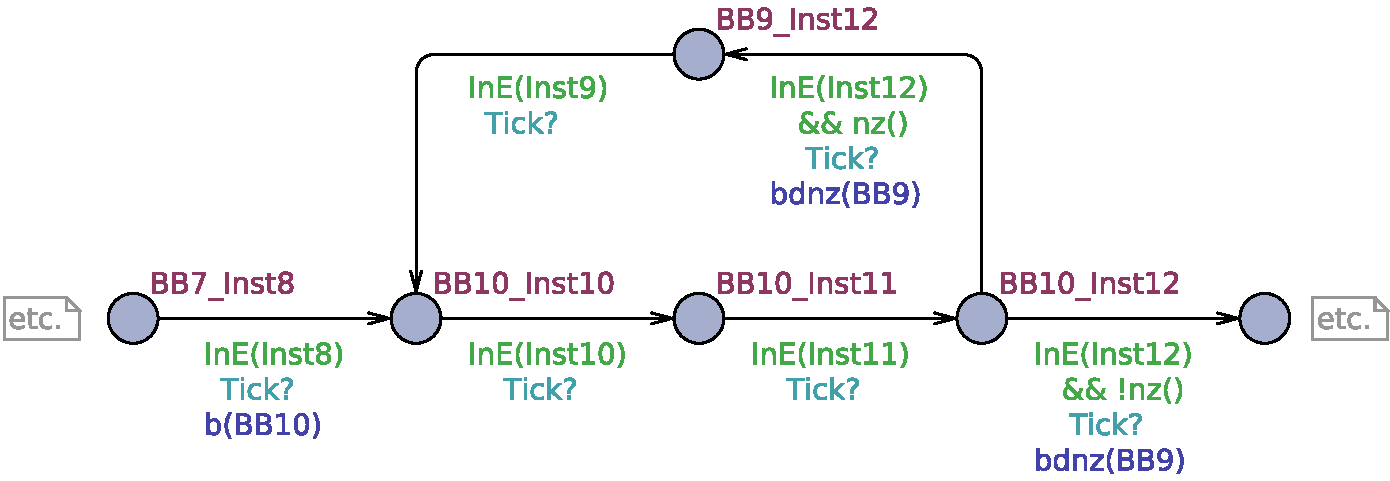
\includegraphics[scale=.5]{fig/program}
      \caption{Part of an automata modeling the functional behavior of a program. The \texttt{bdnz} instruction is a branch instruction that decrements a counter register (\texttt{CTR}) and branches if this counter is not null.}
      \label{fig:program-model}
    \end{figure}

    The label identifies the instruction: thus \texttt{BB$x$\_Inst$y$} denotes the $y^{\text{th}}$ instruction of the $x^{\text{th}}$ basic block of the program.
    %expresses that the next transition to be 
    %taken models the execution of instruction \texttt{Inst$y$} from the basic 
    %block \texttt{BB$x$}, $x$ and $y$ being arbitrary integers.
    The guard \texttt{InE(Inst$y$)} tests if this instruction is currently in the 
    execute stage of the pipeline.
    The \texttt{Tick} signal is used to synchronize the program model with the
    pipeline update.
    The update of the transition calls a UPPAAL function that execute the semantics of the instruction.
    It consists in updating the global variables that model the content of the memory and the status flags of the processor.
    If the instruction is not part of the slice, then the transition does no update as executing its semantics has no influence on the temporal behavior of the system (\textsl{e.g.} the outgoing transition of location
    \texttt{BB10\_Inst10} on fig. \ref{fig:program-model}).
    For conditional branches, two transitions are provided, corresponding to
    the two cases: taken or not taken. 
    For these transitions, the guard is completed with a test to select the
    correct path
    according to the status of the processor (\textsl{e.g.} \texttt{nz()} or
    \texttt{!nz()} on the two outgoing transition of location
    \texttt{BB10\_Inst12} for Inst$12$ on fig. \ref{fig:program-model}).

    %Execution of conditional branching instructions are modeled by two
    %transitions. One transition models the execution the conditional branching 
    %instruction when the condition is satisfied, the other one when the condition
    %is not satisfied. In such case, the \texttt{InE(Inst$y$)} guard is
    %conjuncted with a test checking if the condition is satisfied or not 

    %Due to limitations of BEST, the only indirect branching instructions we are 
    %able to take into account are function return instructions. Our framework do
    %not work for binary code with switch-case statements or function pointers.
    %Execution of return instructions are modeled by one or more 
    %transitions. Each transition models a branch to one of its possible
    %return-sites. In such case, the \texttt{InE(Inst$y$)} guard is conjuncted 
    %with a test selecting the transition to the correct return-site thanks to a 
    %dedicated return-sites stack. This stack is maintained up-to-date through 
    %the execution of the semantics of function call instructions.
  %\textcolor{red}{\bf
    %Afin de correctement expliquer la modélisation, cette partie ajoute des
    %précisions sur la microarchitecture. Ces précisions doivent-elles être
    %déplacées en section 3 ?} \\


  %Figures \ref{fig:incu-model}, \ref{fig:icache-model} \ref{fig:pipeline-model} and \ref{fig:program-model} shows UPPAAL 
  %models. Location labels, invariants, guards, synchronisations and updates are 
  %displayed respectively in purple, pink, green, cyan and blue.
  % Examples for each one of these are, repectively, \texttt{BB7\_Inst8} (fig. 
  % \ref{fig:program-model}), \texttt{clck <= 1} (fig. \ref{fig:pipeline-model}), 
  % \texttt{InE(Inst8)} (fig. \ref{fig:program-model}), \texttt{Tick!} (fig. 
  % \ref{fig:pipeline-model}), \texttt{b(BB10)} (fig. \ref{fig:program-model}).

  \subsection{Modeling the pipeline}
  \label{sec:model:pipeline}

  The model of the pipeline is composed of a set of data structures that capture the content of the internal memory of the components such as the pipeline stages, the instruction buffer and the BTB; and a set of automata used to synchronize the update of this data structures with the flow of time in order to mimic the timing behavior of the system.


    \begin{figure}
      \centering
      \subfloat[][Fetching process control]{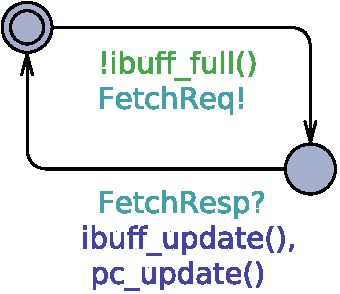
\includegraphics[scale=.5]{fig/incu}\label{fig:incu-model}}
      \qquad\qquad
      \subfloat[][Pipeline execution control]{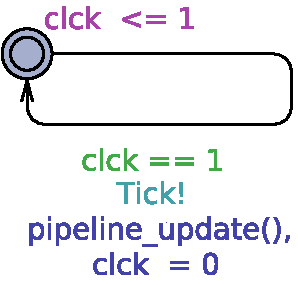
\includegraphics[scale=.5]{fig/pipeline}\label{fig:pipeline-model}}
      \caption{Automata controlling the pipeline.}
    \end{figure}

    The first automaton (figure~\ref{fig:incu-model}) is associated with the (pre)fetching process.
    When the instruction buffer (IBuff) is not full, it tries to fetch an instruction from the instruction cache.
    When an instruction is fetched, the function \texttt{ibuff\_update} updates the instruction buffer and the BTB.
    The instruction buffer is an array of instruction runtime data structures.
    The BTB is a circular buffer with each entry composed of a tag and a 2-bit saturating counter.
    Notice that the target adresses are not actually stored in the BTB because they are already in the program automata.
    The \texttt{pc\_update} updates the PC.
    It performs a BTB lookup in the case of a branch instruction. 
    
    The second automaton (figure~\ref{fig:pipeline-model}) controls the execution of the pipeline. 
    Thanks to the invariant \texttt{clck <= 1} it generates a \texttt{Tick}
    signal every one unit of time. This is used to synchronize the NTA to the frequency of the pipeline.
    It also calls the \texttt{pipeline\_update} function used to update the data structure and variables associated with the pipeline stage following the fetch stage.
    Each pipeline stage is associated with an instruction runtime data structure.
    Updating the stages consists in making instructions progress
    by updating the data structures from stage to stage (including the instruction prefetch buffer), taking into
    account the possible stall cycles due to data or structural hazards.

    Static branch prediction is done when a branch instruction enters the decode stage, if no dynamic branch prediction was available for this instruction at the fetch stage.
    If the prediction is taken, the lower stages are flushed and PC is updated.

    
    %The execution units are in charge of actually executing the instructions.
    %Execution units are the execute, memory access and writeback pipeline
    %stages.

    Branch target resolution is done when a branch instruction enters the execute stage. 
    This encompass a potential BTB update, and, in case of misprediction, a flush of the lower stages and a PC update. 

    %flushed. When resolving dynamic prediction, the BTB is updated according to
    %the outcoming resolution.
    %When a statically predicted branch is resolved as taken, it is inserted in
    %the BTB and the corresponding 2-bit counter is set to the weakly taken
    %value (cf. section \ref{sec:bpbasis}).  

    %As shown on figure \ref{fig:pipeline-model},
    %the pipeline model emits a \texttt{Tick} \textcolor{red}{signal} % Est-ce le terme correct ?
    %every one unit of time and updates the pipeline stages 
    %(\texttt{pipeline\_update()}).
    %This signal is used to synchronise the whole NTA to the frequency of the
    %pipeline.

    %They maintain the PC, the instruction register (IR), the decode pipeline
    %stage, the IBuff and the BTB.
    %The IR stores the next instruction to be fed to the decode stage of the 
    %pipeline.

    %The PC, the IR and decode stage are modeled by an instruction runtime data
    %structures.
    %The instruction prefetch buffer (IBuff) is modeled by an 8-entry array of
    %instruction runtime data structures.
    %The BTB is modeled as a circular buffer by an 8-entry array. Each entry
    %holds a branch instruction address associated with a 2-bit saturating
    %counter. It does not hold the branch instruction target address as this
    %piece of information is already held by the program model. 

    %Static prediction of branch target is done on decode stage.
    %According to the configured static branching prediction policy (AN or BTFN;
    %cf. \ref{sec:architecture:dybrpred}) the branch is predicted taken or not 
    %taken. On taken prediction PC is properly set, the IBuff, IR and are
    %flushed.

    %As shown on figure \ref{fig:incu-model},
    %instruction and control units are modeled by a single TA issuing fetch
    %requests (\texttt{FetchReq!}) for the instruction designated by PC unless 
    %the IBuff is full (\texttt{!ibuff\_full()}).
    %When fetched (\texttt{FetchResp?}), an instruction is either pushed on the
    %IBuff or directly bypassed to the IR if empty (\texttt{ibuff\_update()}).
    %On PC update (\texttt{pc\_update()}) the BTB is queried to check whether the
    %addess of the next instruction to fetch (\textsl{i.e.} the next PC value) can
    %be dynamically predicted or not.

  \subsection{Modeling the memory hierarchy}
  \label{sec:model:memory}

    \begin{figure}
      \centering
      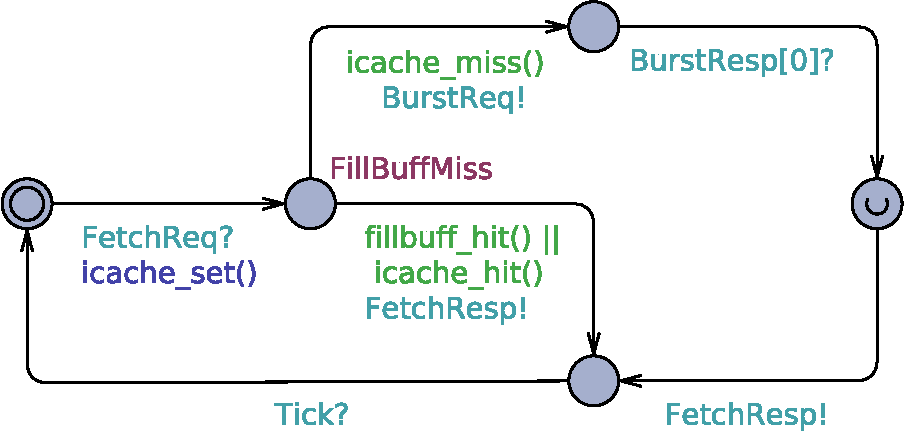
\includegraphics[scale=.5]{fig/icache}
      \caption{Instruction cache access time model.} \vspace{1em}
      \label{fig:icache-model}
    \end{figure}

    The model of the memory hierarchy is composed of a set of data structures and global variables to track the content of the instruction cache and store the content of the useful memory locations (as computed during the program slicing step), and a set of automata to mimic the access times.
    In this paper, we focus on branch prediction so for the sake of clarity we will not give too many details on these models. 

    The automata used to mimic the ICache access time is shown figure~\ref{fig:icache-model}.
    When a fetch request is received, a cache look up and update is performed by the function \texttt{icache\_set}.
    If the instruction is present in the cache or in the fill buffer, the request is acknowledged.
    Otherwise, a request is sent to the Flash memory.
    As explained in section~\ref{sec:architecture:memory}, the instruction cache line fill requires $4\times64$ bits memory transactions from the flash, using a burst access.
%    transfer between the instruction cache and the Flash memory is based on burst of $4\times64$ bits.
    The request is acknowledged before the end of the burst, as soon as the instruction is in the fill buffer. 
    At the end, a synchronization on the \texttt{Tick} signal enforces the cycle required to transfer an instruction from the cache to the fetch stage.



%    The memory unit is in charge of data and instruction memory reads and
    %writes. It maintain the ICache and the ICache fill buffer.

    %The memory unit is modeled by three TAs: a flash memory model, a SRAM
    %model and an ICache model.
    %SRAM accesses are issued for data memory accesses thus
    %the SRAM model is syncrhonised with the pipeline model through the 
    %\texttt{Tick} channel and global variables.
    %Flash and SRAM memory models simply models memory access timings. Flash
    %memory does burst mode access.
    %Flash memory accesses are issued for instruction memory accesses thus the
    %flash memory model is synchronised with the ICache model through 
    %\texttt{BurstReq} and \texttt{BurstResp[$N$]} channels.

    %The ICache is modeled by a TA and a data structure recording a matrix of
    %2 by 64 or 4 by 32 entries of instruction address tags and an interger 
    %corresponding to the global register used by the replacement policy 
    %(cf. \ref{sec:architecture:memory}).
    %Updating the ICache consists of inserting or replacing tags on proper
    %entries of the tag matrix.

    %As shown on figure \ref{fig:icache-model},
    %the ICache model starts by waiting for a fetch request
    %(\texttt{FetchReq?}). On such a request, the ICache data structure in set to
    %process the request for the instruction which address is hold by PC.

    %On ICache hit (\texttt{icache\_hit()}) or ICache fill buffer hit
    %(\texttt{fillbuff\_hit()}) , the model is synchronised with the instruction
    %and control units model on channel \texttt{FetchResp}
    %(cf. \ref{sec:model:btb}).
    %On ICache fill buffer miss, the model execution waits on location 
    %\texttt{FillBuffMiss} until the current burst access returns the queried
    %instruction and then process as a ICache fill buffer hit.
    %On ICache miss, a burst access is requested (\texttt{BurstReq!}). 
    %Upon completion of the first of four burst access (\texttt{BurstReq[0]?}),
    %the instruction requested is stored in the ICache fill buffer and then model
    %can process as a ICache fill buffer hit.



    %\subsubsection{Difference with the e200z4}
      %Our pipeline model does not models the exact behavior of the e200z4 core
      %pipeline.
      %As mentioned in section \ref{sec:architecture:pipeline} the e200z4 is a
      %2-issue superscalar core thus instructions are fetched, decoded and
      %executed by pairs in the pipeline. 
      %We did model a scalar core thus instructions are fetched, decoded and 
      %executed one by one in our pipeline model.
      %Moreover, it is also mentioned that two stages of the pipeline can either
      %be used as two execute stages or two memory stages.
      %We did model separated execute and memory stages.

